\documentclass[font=12pt]{article}
\usepackage{../hdr}
\usepackage{graphics, graphicx}
\newcommand{\mycourse}{02-510 Computational genomics}

\begin{document}

\medskip

\section{Normalization}
\textcolor{red}{RPKM} is a very important normalization tool.\\
\textcolor{blue}{not too sure about tpm, need to double check on that}

\section{Single Cell}
Goals:
\begin{enumerate}
	\item cells differentiates into sub-celltypes
	\item unknown celltype discovery
\end{enumerate}

\subsection{Dimensionality reduction}
Motivation:
\begin{enumerate}
	\item high dim data often has lower dim representation w/o much reconstruction error
	\item lower dim representation can often represent info about high dim pairwise dist.
\end{enumerate}
Types of dim-red:
\begin{itemize}
	\item \textcolor{red}{Global methods}
		\begin{enumerate}
			\item all pairwise dist equally impt
			\item lower dim pairwise dist fit high-dim ones
			\item often use magnitude or rank order
		\end{enumerate}
	\item \textcolor{red}{Local methods}
		\begin{enumerate}
			\item only local dist reliable in high dim
			\item more weight on modelling local dist correctly
		\end{enumerate}
\end{itemize}
Methods:
\begin{itemize}
	\item PCA
		\begin{itemize}
			\item finds directions with largest variance
			\item minimize squared reconstruction error
			\item equiv to liner autoencoders
			\item Steps of PCA
			\begin{enumerate}
				\item $\overline{X}$: mean of all samples(usually rows), adjust $ X \rightarrow X' = X - \overline{X}$ 
				\item covar matrix $ C = X'^T X'$
				\item find eigenvectors and eigenvalues of $C$, ie. all pair of $\vec{v}, \lambda$ st. $ C\vec{v} = \lambda \vec{v}$
				\item eigenvalues can be used to calculate percentage of total variance for each component \[v_j = 100\frac{\lambda_j}{total \quad eigenvalue}\] 
			\end{enumerate}
		\end{itemize}
		\textcolor{blue}{This is non-parametric method, do not insist on a parametric encoding function}
	\item Multi-Dimensional Scaling
		\begin{itemize}
			\item  arrange low dim points to minimize diff between pairwise distances in the high and low D space
			\item a possible approach: start w a random vector, perform gradient decent
			\item \textcolor{red}{is there something to do with PCA?} then we don't need iterative method
		\end{itemize}
	\item Sammon (non-linear autoencoder)
		\begin{itemize}
			\item  with extra layers, much more powerful than PCA, but can be slow to converge, and can get stuck on local optima
			\item Multi-Dimensional Scaling(MDS) can be made non-linear by giving higher weights to smaller distances, a popular formula is 
				\[ cost = \sum_{ij} \left(\frac{|x_i - x_j| - |y_{i}-y_j|}{|x_i - x_j|}\right)^2\]
				where $ x$ is high-dim dist, and  $y$ is low-dim dist
			\item still slow and get stuck on local optima
		\end{itemize}
\end{itemize}

\subsection{Graph-basd method}
		\begin{itemize}
			\item address uniform circularity
			\item  \textcolor{red}{Isomap} is a dim-red technique based on graphs
				\begin{itemize}
					
			\item each datapoint is connected to $k$ nearest neighbor in high-dim
			\item edge weights = euclidean dist
			\item approx of distance = shortest path in contracted graph
			\end{itemize}
		\item \textcolor{red}{Probabilistic local MDS}
			\begin{itemize}
				\item local distances are more impt than non-local ones
				\item in this way all local distances are given equal importance	\end{itemize}

		\item \textcolor{red}{stochastic neighbor embedding(SNE)} has a probabilistic way to decide if a distance is local
			\begin{itemize}
				\item convert global distances into probability of one datapoint picking another datapoint as its neighbor \textcolor{blue}{(what defines a neighbor tho) - still about isomaps?}
				\item each point in high-dim has a conditional probability of picking any other point as its neighbor
			\item distribution (some sort of Gaussian) is over high-dim distances (if high-dim coords unavailable, a similarity / dissimilarity matrix may be used)\\ $p_{j|i}$ is the prob. of picking j given starting at i in high-dim.
				\[ P_{j|i} = \frac{e^{-2d_{ij}^2 / 2\sigma_i^2}}{\sum_k e^{{-d_{ik}^2}/{2\sigma_i^2}}} \]
				\item having the probabilities potentially allow us to throw away the raw high-dimensional data
				\item evaluation done using pairwise distance in low dimensional map (shows how well the lower dim representation models high-dim data ig)\\
					$q_{j|i}$ is the prob of picking j given starting at i in low-dim
				\item compute the \textcolor{red}{Kullback-Leibler divergence} between prob. in the high-dim and low-dim spaces \textcolor{blue}{(why not just use dist in high dim?) - more space / time efficient}
				\item nearby pts in high-dim should be close in low-dim
			\end{itemize}
		\item picking $\sigma$ used to compute  $p$ - the radius of the gaussian
			 \begin{itemize}
				 \item different radius is needed in different parts of the space to keep the no. of neighbors constant
				 \item big radius $\rightarrow$ high entropy for distribution over i's neighbors
				 \item small radius $\rightarrow$ low entropy
				
			\end{itemize}
		\item \textcolor{red}{Symmetric SNE}
			\begin{itemize}
				\item simpler than stochastic
				\item works best if different procedures are used for computing $p$'s and  $q$'s.
				\item compromise: no longer guarantees that if using same dimension will produce optimal solution
				\item turn conditional prob into symmetric pairwise probabilities
			\end{itemize}
		\item Optimization methods for SNE
			\begin{itemize}
				\item simulated annealing could lead to better global optimization
				\item add Gaussian noise to $y$ location in each update
				\item spend longer time at noise level where global structure start to form
				\item \textcolor{red}{t-SNE} - use Gaussian at many (infinite) spatial scales, cheaper as we don't have to exponentiate anymore \textcolor{blue}{(why????)} 
			\end{itemize}
				\end{itemize}
\subsection{Supervised dim-red: Neural networks}
\begin{itemize}
	\item last few layers have much fewer values than inputs
	\item use intermediate layers as lower-dim representations
	\item can easily add prior biological knowledge, such as protein interactions or transcription factors
	\item essentially, some nodes in the hidden layer are same as before, others are based on biological info
\end{itemize}
\subsubsection{Additional NN architecture: Siamese}
\begin{itemize}
	\item supervised, but not trying to maximize training accuracy
	\item input: whether each pair is similar
	\item output: binary label of similar / not similar
	\item thus directly optimize dim-red layer for KNN
\end{itemize}
\newpage
\section{ChIP-Seq}
\subsection{Background}
\begin{itemize}
	\item transcription factors bind to specific locations on the chromosome
	\item the binding is highly specific
	\item this has impact on gene regulation
	\begin{figure}[h!]
		\centering
		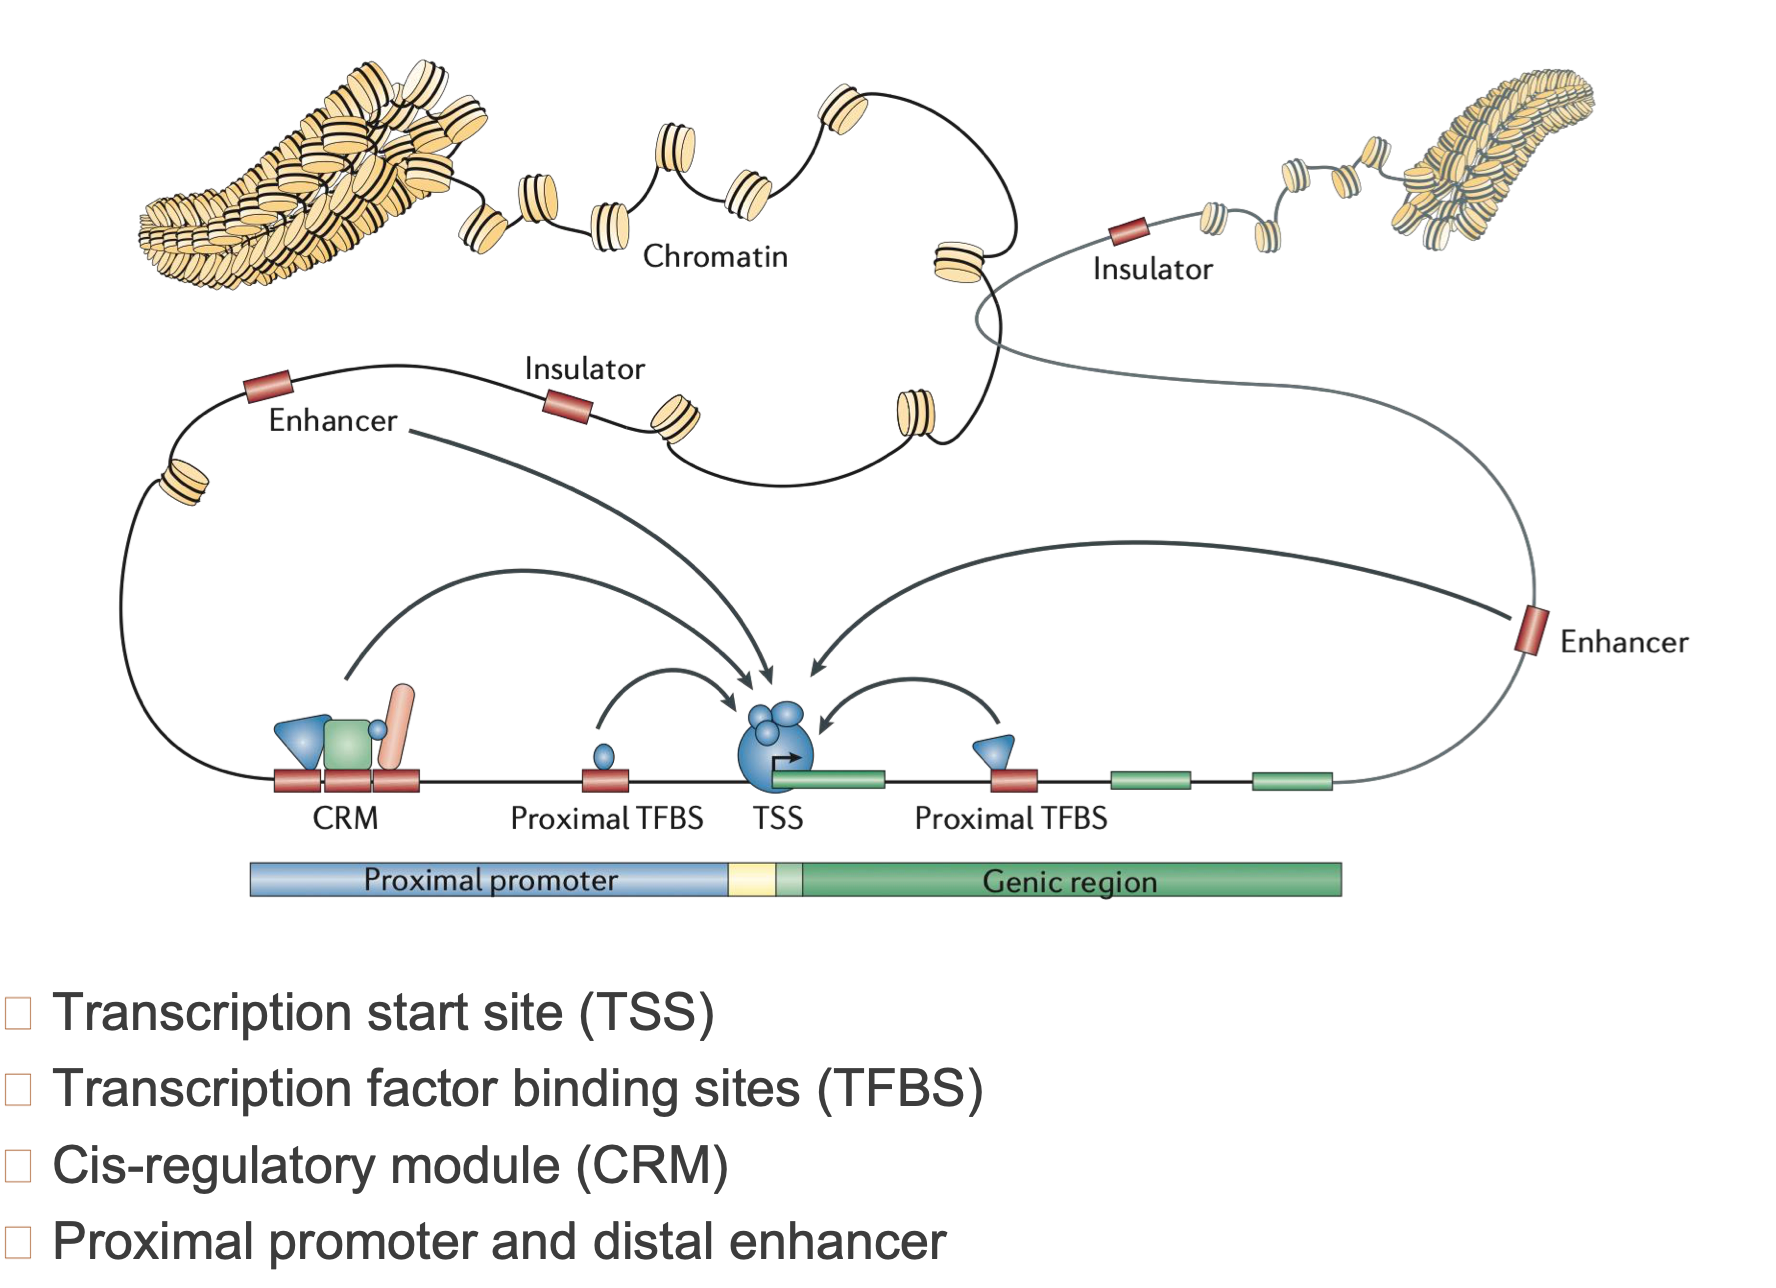
\includegraphics[width=0.6\linewidth]{TFillustration}
		\label{fig:tfillustration}
	\end{figure}
	\item The core promotor regions has about 300 TF, \\
	(general transcription machinery, required for the transcription of most things), \\
	another 1500 TFs for others (proximal enhancer/promotor/silencer, only affect some genes)
	\item comparisons of different whole genome enrichment technologies
	\begin{figure}[h!]
		\centering
		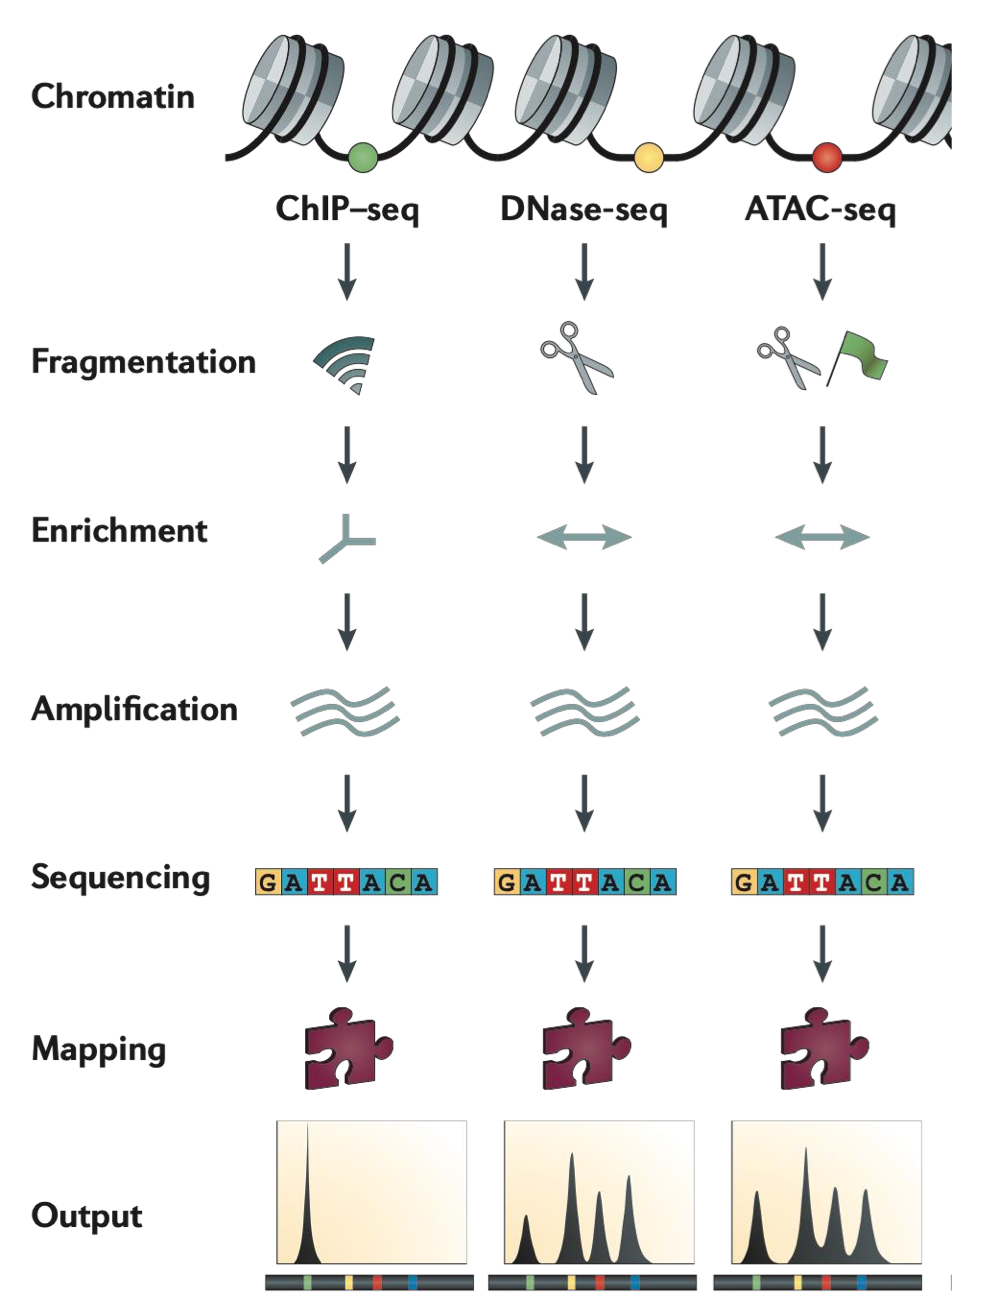
\includegraphics[width=0.4\linewidth]{genomewide_profiling_tech}
		\label{fig:genomewideprofilingtech}
	\end{figure}
	
\end{itemize}
\subsection{Questions related to TF binding}
\begin{itemize}
	\item Where do they bind
	\begin{itemize}
		\item some almost always bind to proximal promotors
		\item others could bind to many regions
	\end{itemize}
	\item How does specific binding work
	\begin{itemize}
		\item exists a consensus motif (most common sequence)
		\item looks like this 
		\begin{figure}[h!]
			\centering
			
\includegraphics[scale=0.2]{concensusmotif}
			\label{fig:concensusmotif}
		\end{figure}
		\item shows which nucleotide is most abundant at each position, represented as \kyw{Position Weight Matrix (PWM)}
		\item \textcolor{red}{Motif}: a \kyw{recurring} sequence with biological importance
			\begin{itemize}
				\item can be constant or have a feww variable elements
				\item often serves as binding site for TFs /proteins
				\item often very short (5-25)
				\item often distant from gene
				\item  often has inexact repeating pattern (challenge for identification)
			\end{itemize}
		\item sometimes also an effect of protein-protein interactions,\\
			ie. protein conformation change upon interactions etc?
		\item to determine binding site, often uses \textcolor{red}{Protein Weight Matrix}, but it is over-simplifying
		\end{itemize}
	\item How to identify where they bind
		\begin{itemize}
			\item genes regulated by the same TF are likely to have the same motif in regulatory region
			\item to find genes regulated by the same TF $\rightarrow$ \cmt{comparative genomics} could be very useful
			\item eg. knock-off of specific TFs $\rightarrow$ lower expression of a set of genes
			\item group of genes that are co-expressed across many set of experiments are also likely to be regulated by same TF
			\item challenges
				\begin{itemize}
					\item we don't know the exact motif seq
					\item we don't know how far it will be
					\item motifs can differ slightly across
					\item how to distinguish it from just ``random'' sequences that happen to repeat?
				\end{itemize}
			\item Multiple sequence alignment (MSA)
			\item motif-finding based on EM algorithm (MEME-suite - Multiple EM for Motif Elucidation)
		\end{itemize}
	\item How is it involved in gene regulation
	\item Is it useful for gene regulatory network?
\end{itemize}
\subsection{ChIP-seq}
\begin{itemize}
	\item technology:\\
	\kyw{ChIP}: chromatin immunoprecipitation\\
	studies protein interaction with DNA\\
	able to map global binding site precisely for any protein of interests
		\begin{enumerate}
			\item chromatin immunoprecipitation + high throughput sequencing
			\item detect genome-wide location of TF and other binding proteins in labs
			\item find all DNA seq bound by TF-X
			\item try to learn the regulatory mechanisms of a TF or DNA-binding protein
		\end{enumerate}
	\item General strategies to call ChIP-seq peaks
		\begin{itemize}
			\item ChIP-seq yields distributions for tags from forward and reverse strands
			\item overlap of the two can be observed
			\item actual binding site of TF should be between the 2 distributions
			\item from the difference between the 2 peaks $\rightarrow$ formulate a single \kyw{peak summit}  
		\end{itemize}
	\item MACS: model-based analysis for ChIP-seq
	\begin{enumerate}
		\item map reads using Bowtie2
		\item get ChIP-seq reads around but may not contain binding site
		\item sequence are from ends of randomly chopped segments $->$ hopefully overlap at binding site
		\item produce 2 adj. set of read peaks located about $ 2\times $ fragment length away
		\item \kyw{shift distance}: dist between read peaks at which will find true peak
		\item automatically subtract control to define a final set of peaks
	\end{enumerate}
	\begin{itemize}
		\item input: \\
		bandwidth : sonication size\\
		mfold: high-confidence fold enrichment
		\item slides $ 2\times $ bandwidth window across genome to find regions with tags $ > mfold$ enriched compared to a random tag
		\item random sample 1000 high quality peaks, separate their Watson Crick tags, and align by midpoint $->$ 2 peaks, shifts = $ d/2 $
		\item tag distribution $ ~ Poisson $
		\item MACS uses a dynamic parameter $ \lambda_{local} $
		\item \cmt{P-val of peaks?}
		\item \cmt{FDR?}
	\end{itemize}
	\item Downstream analysis
	\begin{itemize}
		\item to identify motif for TF using ChIP-seq peaks -- \kyw{MEME}
		\item to find out what the sequence motifs resembles -- \kyw{TomTom}
		\item to find peak regions of known motifs -- \kyw{FIMO}
		\item look up biological pathways or functions of target genes of TF --\kyw{GREAT}
	\end{itemize}
	\item Practical pipeline
	
\end{itemize}

\newpage
\section{cis-regulatory motif}


\newpage
\section{Haplotype inference}
\subsection{Phase}
\begin{figure}[h!]
	\centering
	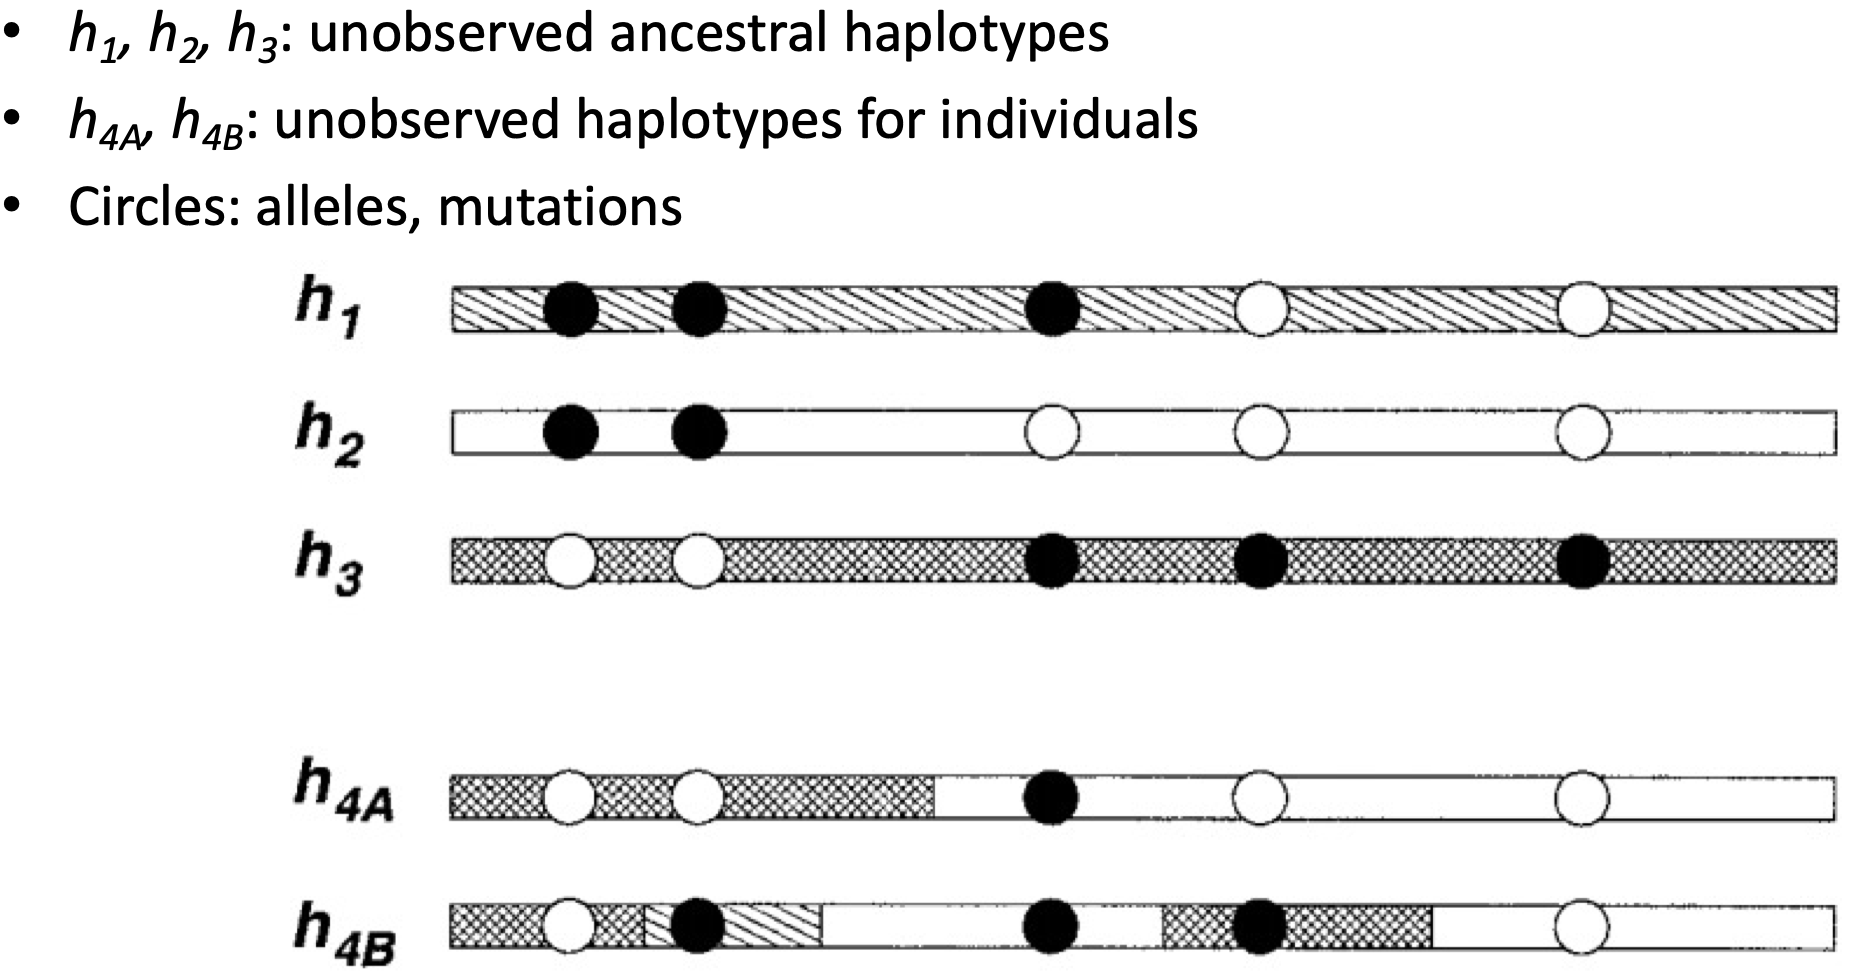
\includegraphics[width=0.7\linewidth]{phase}
	\caption{}
	\label{fig:phase}
\end{figure}

\begin{figure}[h!]
	\centering
	\includegraphics[width=0.7\linewidth]{"haplotype structure"}
	\label{fig:haplotype-structure}
\end{figure}
\begin{itemize}
	\item Genotype inputation
	\begin{itemize}
		\item Given: SNP array genotype data
		\item some has missing data / untyped SNPs
		\item much cheaper
		\item use HMM
		\item more data, more acurate for inputation
	\end{itemize}
	\item Beagle / SHAPE-IT are most commonly used software
\end{itemize}
\subsection{Linkage disequilibrium (LD)}
\begin{itemize}
	\item reflect rs between alleles at diff loci
	\begin{itemize}
		\item linkage equilibrium: no linkage, not coupled
		\item disequilibrium $ \rightarrow $ linkage
	\end{itemize}
	\item \kyw{LD:} allelic association meansure
	\item calculating LD:
	\begin{itemize}
		\item assume independence, calculate expected frequency
		\item $ D_{AB} = P_{AB} - P_A P_B $
	\end{itemize}
	\item calculate for all loci (SNPs)
	\item spot-light figures\begin{figure}[h!]
		\centering
		\includegraphics[scale = 0.2]{"chromosome spotlight"}
		\label{fig:chromosome-spotlight}
	\end{figure}
	\item neighboring loci shows more linkage\\
	there could be LP blocks on the chromosome, where there's stronger linkage within block and weaker across block\\
	each block is like a voting district / \kyw{Marker regions}
	\item They are \cmt{Tag SNPs}
	\item pretty standard practice
	\item dense genotyping more expensive 
	\begin{itemize}
		\item get the LP
		\item use inference on sparser genotyping 
		\item multi-phase procedure
	\end{itemize}
\end{itemize}

\section{Population structure}
\subsection{Background}
\begin{itemize}
	\item def: set of individuals with distinct genetic variations
	\item eg. ancestral history, lactose intolerance
	\item Hardy-Weinburg equilibrium
	\begin{itemize}
		\item Under random mating, both allele and genotype frequency remain const
		\item Current gen:
		\begin{itemize}
			\item $ D + H + R = 1 $
			\item $ p = \frac{2D + H}{2} $
			\item $ q = \frac{2R + H}{2} $
		\end{itemize}
		\item Next gen:
		\begin{itemize}
			\item $ D' = p^2 $
			\item $ H' = 2pq $
			\item $ R' = q^2 $
			\item $ p' = \frac{2p^2 + 2pq}{2} = p^2 + pq = p $
			\item $ q' = \frac{2p^2 + 2pq}{2} = q^2 + pq = q$
		\end{itemize}
		\item given population data, can test if it holds (often chi-square test)
		\begin{itemize}
			\item testing is recommended
			\item if fail, means something is going on
			\item or genotyping error
			\item want HWE to hold for control group
		\end{itemize}
		\begin{enumerate}
			\item compute allele freq from observed data
			\item compute expected genotype freq
			\item compute test statistic (deg of freedom 1)
		\end{enumerate}
		\item Due to \kyw{Genetic drift}, even when assumptions of HWE hold, HWE may not hold
	\end{itemize}
	\item genetic drift
	\begin{itemize}
		\item change in allele freq due to random sampling
		\item all mutations eventually drift to 0 or 1 eventually
		\item is neutral
	\end{itemize}
	\item Wright's $ F_{ST} $ (Wright-Fisher model)\\
	\[ {{2N}\choose{k}} p^k q^{2N-k} \]
	\item Ways how populations evolve
	\begin{itemize}
		\item population divergence\\
		separated into subpopulations with independent selection and drift
		\item admixture\\
		mixing of population
	\end{itemize}
\subsection{Infering pop structure from genotype data (nowadays mostly just PCA)}
Mixture model 
\begin{itemize}
	\item cluster individual into K populations
	\item does not model admixture
	\item cluster individual into populations
	\item probability model for mixture of $ C $ Gaussians
	\[ p(x) = \sum_{i=1}^k p(x|c=i)\cdot p(c=i)\]
	\item $ c $: labels, $ p(c) $ label freq, multinuilli
	\item $ x $: genotype / alleles, $ p(x|c) = \Pi_{i=1}^j p(x_i|c)$ , assume independence
	\item can then learn the model with EM
	\item Inference: $p(c|x)$ to infer cluster label
\end{itemize}
Admixture model
\begin{itemize}
	\item 
\end{itemize}
\end{itemize}




\end{document}
